% Build: lualatex -interaction=nonstopmode -halt-on-error main.tex
\documentclass[12pt,a4paper]{article}

\usepackage{fontspec,polyglossia}
\setdefaultlanguage{ukrainian}
\setmainfont{NewCM10-Regular.otf}[
  BoldFont=NewCM10-Bold.otf,
  ItalicFont=NewCM10-Italic.otf,
  BoldItalicFont=NewCM10-BoldItalic.otf
]
\setsansfont{Noto Sans}
\setmonofont{Noto Sans Mono}[Scale=0.82]

\usepackage{xurl}
\usepackage{geometry,graphicx,booktabs,array,enumitem,caption,titlesec,xcolor,fvextra,float}
\geometry{left=2cm,right=2cm,top=2cm,bottom=2cm}
\setlength{\parindent}{1.25cm}
\setlength{\parskip}{4pt}
\setlength{\emergencystretch}{3em}
\linespread{1.08}
\titleformat{\section}{\normalfont\fontsize{14}{16}\selectfont\bfseries}{\thesection}{0.6em}{}
\titleformat{\subsection}{\normalfont\fontsize{12}{14}\selectfont\bfseries}{\thesubsection}{0.6em}{}
\captionsetup{hypcap=false,font=small,labelfont=bf,labelsep=endash}
\DefineVerbatimEnvironment{code}{Verbatim}{fontsize=\footnotesize,breaklines=true,breakanywhere=true,frame=single,framesep=2mm}

\usepackage[
  unicode,
  colorlinks=true,
  linkcolor=black,
  urlcolor=blue,
  pdfauthor={Давидчук Артем},
  pdftitle={Архітектура комп'ютерів. Частина 2. Лабораторна робота №5}
]{hyperref}

\begin{document}

\pagenumbering{gobble}
\begin{titlepage}
  \begin{center}
    
\includegraphics[width=0.7\textwidth]{../../../../../../templates/letterhead.png}\\[1em]
    \large
    Національний технічний університет України\\
    «Київський політехнічний інститут імені Ігоря Сікорського»\\[1em]
    Факультет інформатики та обчислювальної техніки\\
    Кафедра обчислювальної техніки
  \end{center}

  \vfill
  \begin{center}
    \textbf{\LARGE Архітектура комп'ютерів}\\[0.4em]
    \textbf{\Large Частина 2. Процесори}\\[2em]
    \textbf{\Large Лабораторна робота №5}\\[0.7em]
    \parbox{0.9\textwidth}{\centering
      «Взаємодія завантажуваних модулів ядра Linux»}
  \end{center}

  \vfill
  \begin{flushright}
    Виконав: студент групи ІО-41\\
    \textit{Давидчук Артем}\\[1em]
    Перевірив: \textit{Каплунов А.~В.}
  \end{flushright}

  \vfill
  \begin{center}Київ --- 2026\end{center}
\end{titlepage}
\pagenumbering{arabic}

\section{Мета роботи}

Ознайомитися з експортом символів і залежностями між завантажуваними
модулями ядра Linux. Навчитися організовувати спільний заголовковий файл,
додавати каталог заголовків до Kbuild, вимірювати тривалість операцій за
допомогою \texttt{ktime\_t} та перевіряти модулі в QEMU для ARMv7.

\section{Постановка задачі}

Реалізацію з лабораторної роботи №4 потрібно розділити на модулі
\texttt{hello1} та \texttt{hello2}. Перший модуль експортує функцію
\texttt{print\_hello()}, зберігає події у списку та вимірює час кожного
друку. Другий модуль містить параметр \texttt{count} і викликає експортовану
функцію задану кількість разів.

Спільний заголовок \texttt{hello1.h} необхідно розмістити у підкаталозі
\texttt{inc}. Для підключення його лише за іменем у Kbuild використовується
\texttt{ccflags-y}. Повідомлення ядра мають формуватися через
\texttt{pr\_info()}, \texttt{pr\_warn()} і \texttt{pr\_err()}.

Потрібно перевірити всі варіанти параметра, порядок завантаження модулів і
спробу завантажити \texttt{hello2.ko} без \texttt{hello1.ko}.

Репозиторій із вихідним кодом і Makefile:
\begin{center}
\href{https://github.com/davidchyk/university_roadmap/tree/main/semester5/ca2/work/labs/lab5}{github.com/davidchyk/university\_roadmap/.../ca2/work/labs/lab5}
\end{center}

\section{Теоретичні відомості}

\subsection{Експорт символів і залежність модулів}

Функції одного модуля за замовчуванням недоступні іншим модулям.
Макрос \texttt{EXPORT\_SYMBOL(print\_hello)} додає функцію до таблиці
експортованих символів ядра. Під час збирання modpost знаходить використання
цього символу в \texttt{hello2} та записує залежність від \texttt{hello1}.
Тому \texttt{modinfo hello2.ko} показує поле \texttt{depends: hello1}.

Команда \texttt{insmod} не завантажує залежності автоматично. Якщо
\texttt{hello2.ko} вставити першим, ядро не може розв'язати посилання на
\texttt{print\_hello} і повертає помилку \texttt{Unknown symbol}.

\subsection{Kbuild і спільний заголовок}

Обидва модулі підключають заголовок однаково:

\begin{code}
#include "hello1.h"
\end{code}

Каталог \texttt{inc} додається до параметрів компілятора через змінну
\texttt{ccflags-y}. Директива \texttt{\$(src)} містить абсолютний шлях до
каталогу вихідних файлів модуля під час роботи Kbuild.

\begin{code}
ccflags-y := -I$(src)/inc
obj-m := hello1.o hello2.o
\end{code}

\subsection{Вимірювання часу та список ядра}

Кожен елемент списку містить дві часові мітки: до і після виклику
\texttt{pr\_info()}. Тривалість обчислюється як
\texttt{ktime\_sub(finish, start)} та переводиться в наносекунди функцією
\texttt{ktime\_to\_ns()}. Під час вивантаження \texttt{hello1} список
обходиться безпечним макросом \texttt{list\_for\_each\_entry\_safe()}, а
пам'ять кожного елемента звільняється через \texttt{kfree()}.

\section{Програмна реалізація}

\subsection{Модуль hello1}

Структура події містить вузол списку та дві часові мітки:

\begin{code}
struct hello_event {
    struct list_head list;
    ktime_t start;
    ktime_t finish;
};
\end{code}

Функція \texttt{print\_hello()} виділяє пам'ять, фіксує час до та після
друку, додає подію до списку й експортується для інших модулів:

\begin{code}
event->start = ktime_get();
pr_info("Hello, world!\n");
event->finish = ktime_get();
list_add_tail(&event->list, &event_list);

EXPORT_SYMBOL(print_hello);
\end{code}

Під час вивантаження для кожної події друкується фактична тривалість:

\begin{code}
pr_info("print duration: %lld ns\n",
        (long long)ktime_to_ns(ktime_sub(event->finish,
                                        event->start)));
\end{code}

\subsection{Модуль hello2}

Параметр перенесено до другого модуля. Значення за замовчуванням дорівнює
1; для 0 і діапазону 5--10 виводиться попередження; значення понад 10
спричиняє повернення \texttt{-EINVAL}.

\begin{code}
static unsigned int count = 1;
module_param(count, uint, 0444);
MODULE_PARM_DESC(count, "Number of calls to print_hello");

for (i = 0; i < count; i++) {
    error = print_hello();
    if (error)
        return error;
}
\end{code}

\section{Збирання і перевірка стилю}

Використано ядро Linux 4.19.325 і GNU Arm Toolchain 8.3-2019.03. Для
кроскомпіляції встановлено \texttt{ARCH=arm} і
\texttt{CROSS\_COMPILE=arm-eabi-}. Перевірка \texttt{checkpatch.pl}
виконана для \texttt{hello1.c}, \texttt{hello2.c} та
\texttt{inc/hello1.h}. У всіх випадках отримано
\texttt{0 errors, 0 warnings}.

Команда \texttt{file} визначила обидва файли \texttt{.ko} як 32-бітні
ARM EABI5 relocatable ELF. Поле \texttt{vermagic} дорівнює
\texttt{4.19.325 SMP mod\_unload ARMv7 p2v8}. У
\texttt{Module.symvers} присутній експортований символ
\texttt{print\_hello}, а \texttt{modinfo hello2.ko} показує залежність
\texttt{hello1} та параметр \texttt{count} типу \texttt{uint}.

\begin{figure}[H]
  \centering
  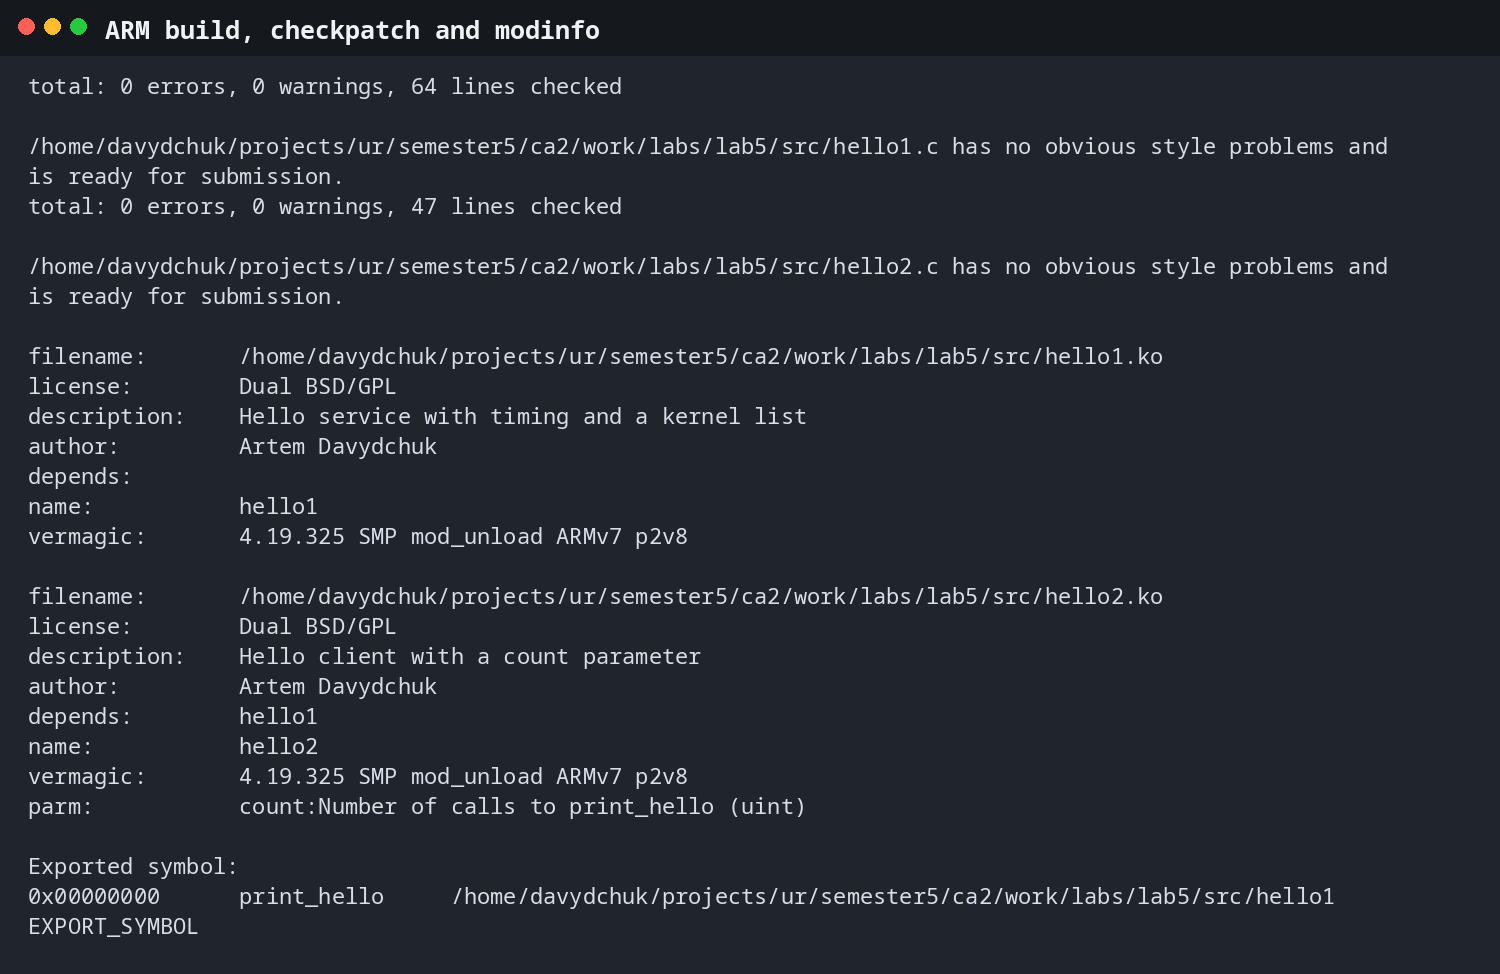
\includegraphics[width=\textwidth]{media/build-and-modinfo.png}
  \caption{Перевірка стилю, modinfo та експортований символ}
\end{figure}

\section{Запуск у QEMU}

До окремої копії initramfs додано \texttt{hello1.ko} і
\texttt{hello2.ko}. Початковий архів із ЛР №3 не змінювався. Система
запускалася командою:

\begin{code}
qemu-system-arm \
  -machine virt -m 512 -nographic \
  -kernel "$HOME/bbb-lab/repos/busybox/_install/boot/zImage" \
  -initrd build/initramfs/rootfs-lab5.cpio.gz \
  -append "root=/dev/ram0 rw console=ttyAMA0,115200 mem=512M"
\end{code}

Ядро визначило архітектуру \texttt{armv7l} і версію 4.19.325. Значення
встановленого параметра перевірялося через файл
\path{/sys/module/hello2/parameters/count}.

\section{Результати перевірки}

\subsection{Перевірка залежності}

Спроба виконати \texttt{insmod hello2.ko} до завантаження
\texttt{hello1.ko} завершилася статусом 1. У журналі ядра зафіксовано
\texttt{Unknown symbol print\_hello (err -2)}, а \texttt{lsmod} підтвердив,
що \texttt{hello2} не завантажено. Після правильного порядку
\texttt{hello1}, потім \texttt{hello2}, обидва модулі з'явилися у
\texttt{lsmod}; для \texttt{hello1} показано користувача \texttt{hello2}.

\begin{figure}[H]
  \centering
  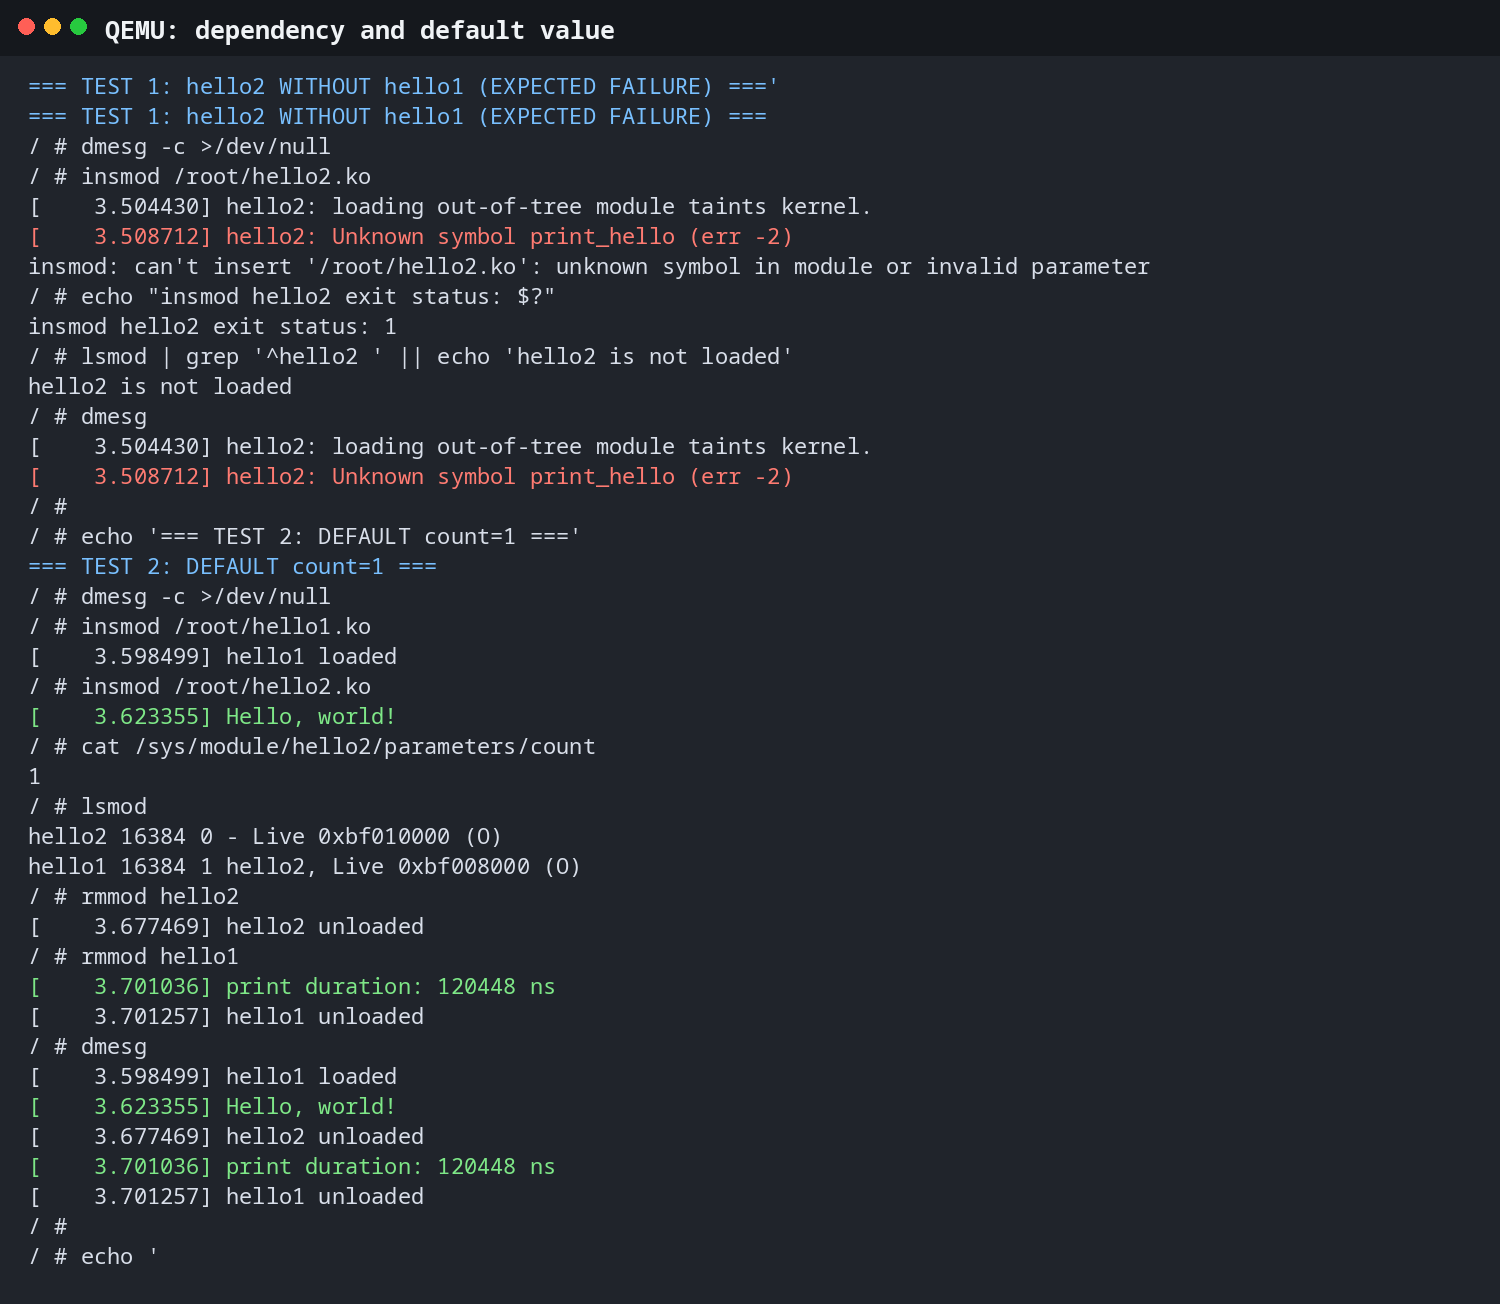
\includegraphics[width=0.72\textwidth]{media/dependency-and-default.png}
  \caption{Невдале завантаження без залежності та успішний типовий запуск}
\end{figure}

\subsection{Перевірка параметра}

\begin{table}[H]
\centering
\small
\begin{tabular}{c p{0.31\textwidth} p{0.43\textwidth}}
\toprule
\textbf{count} & \textbf{Результат} & \textbf{Спостереження}\\
\midrule
не задано & успішне завантаження & одне привітання; sysfs містить 1; один вимір тривалості\\
0 & успішне завантаження & попередження; привітання та виміри відсутні; sysfs містить 0\\
3 & успішне завантаження & три привітання і три значення тривалості; sysfs містить 3\\
7 & успішне завантаження & попередження; сім привітань і сім значень тривалості\\
11 & відмова, статус 1 & повідомлення \texttt{pr\_err}; \texttt{-EINVAL}; hello2 відсутній у lsmod\\
\bottomrule
\end{tabular}
\caption{Результати тестування параметра count}
\end{table}

\begin{figure}[H]
  \centering
  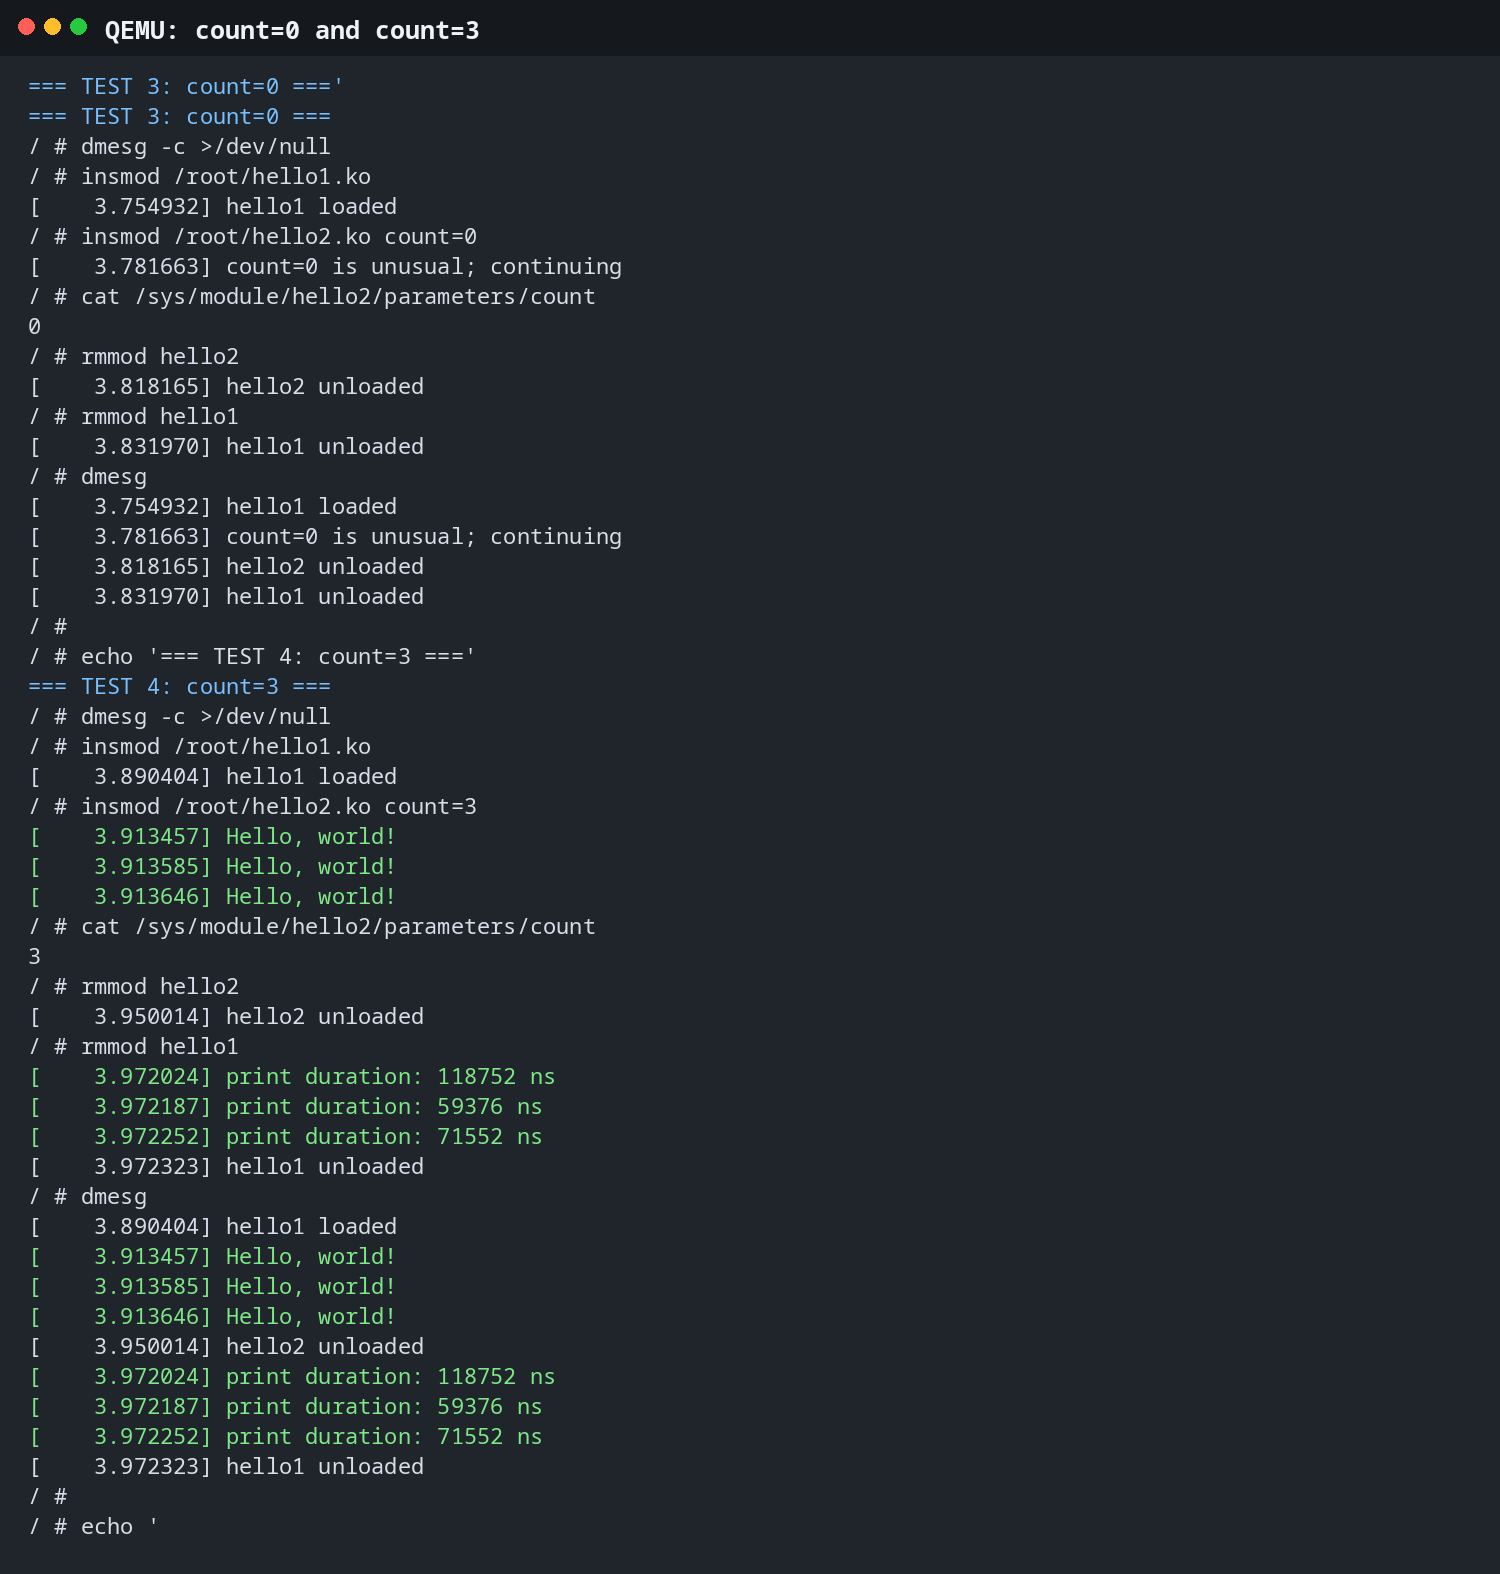
\includegraphics[width=0.69\textwidth]{media/parameters-0-3.png}
  \caption{Перевірка значень count=0 і count=3}
\end{figure}

\begin{figure}[H]
  \centering
  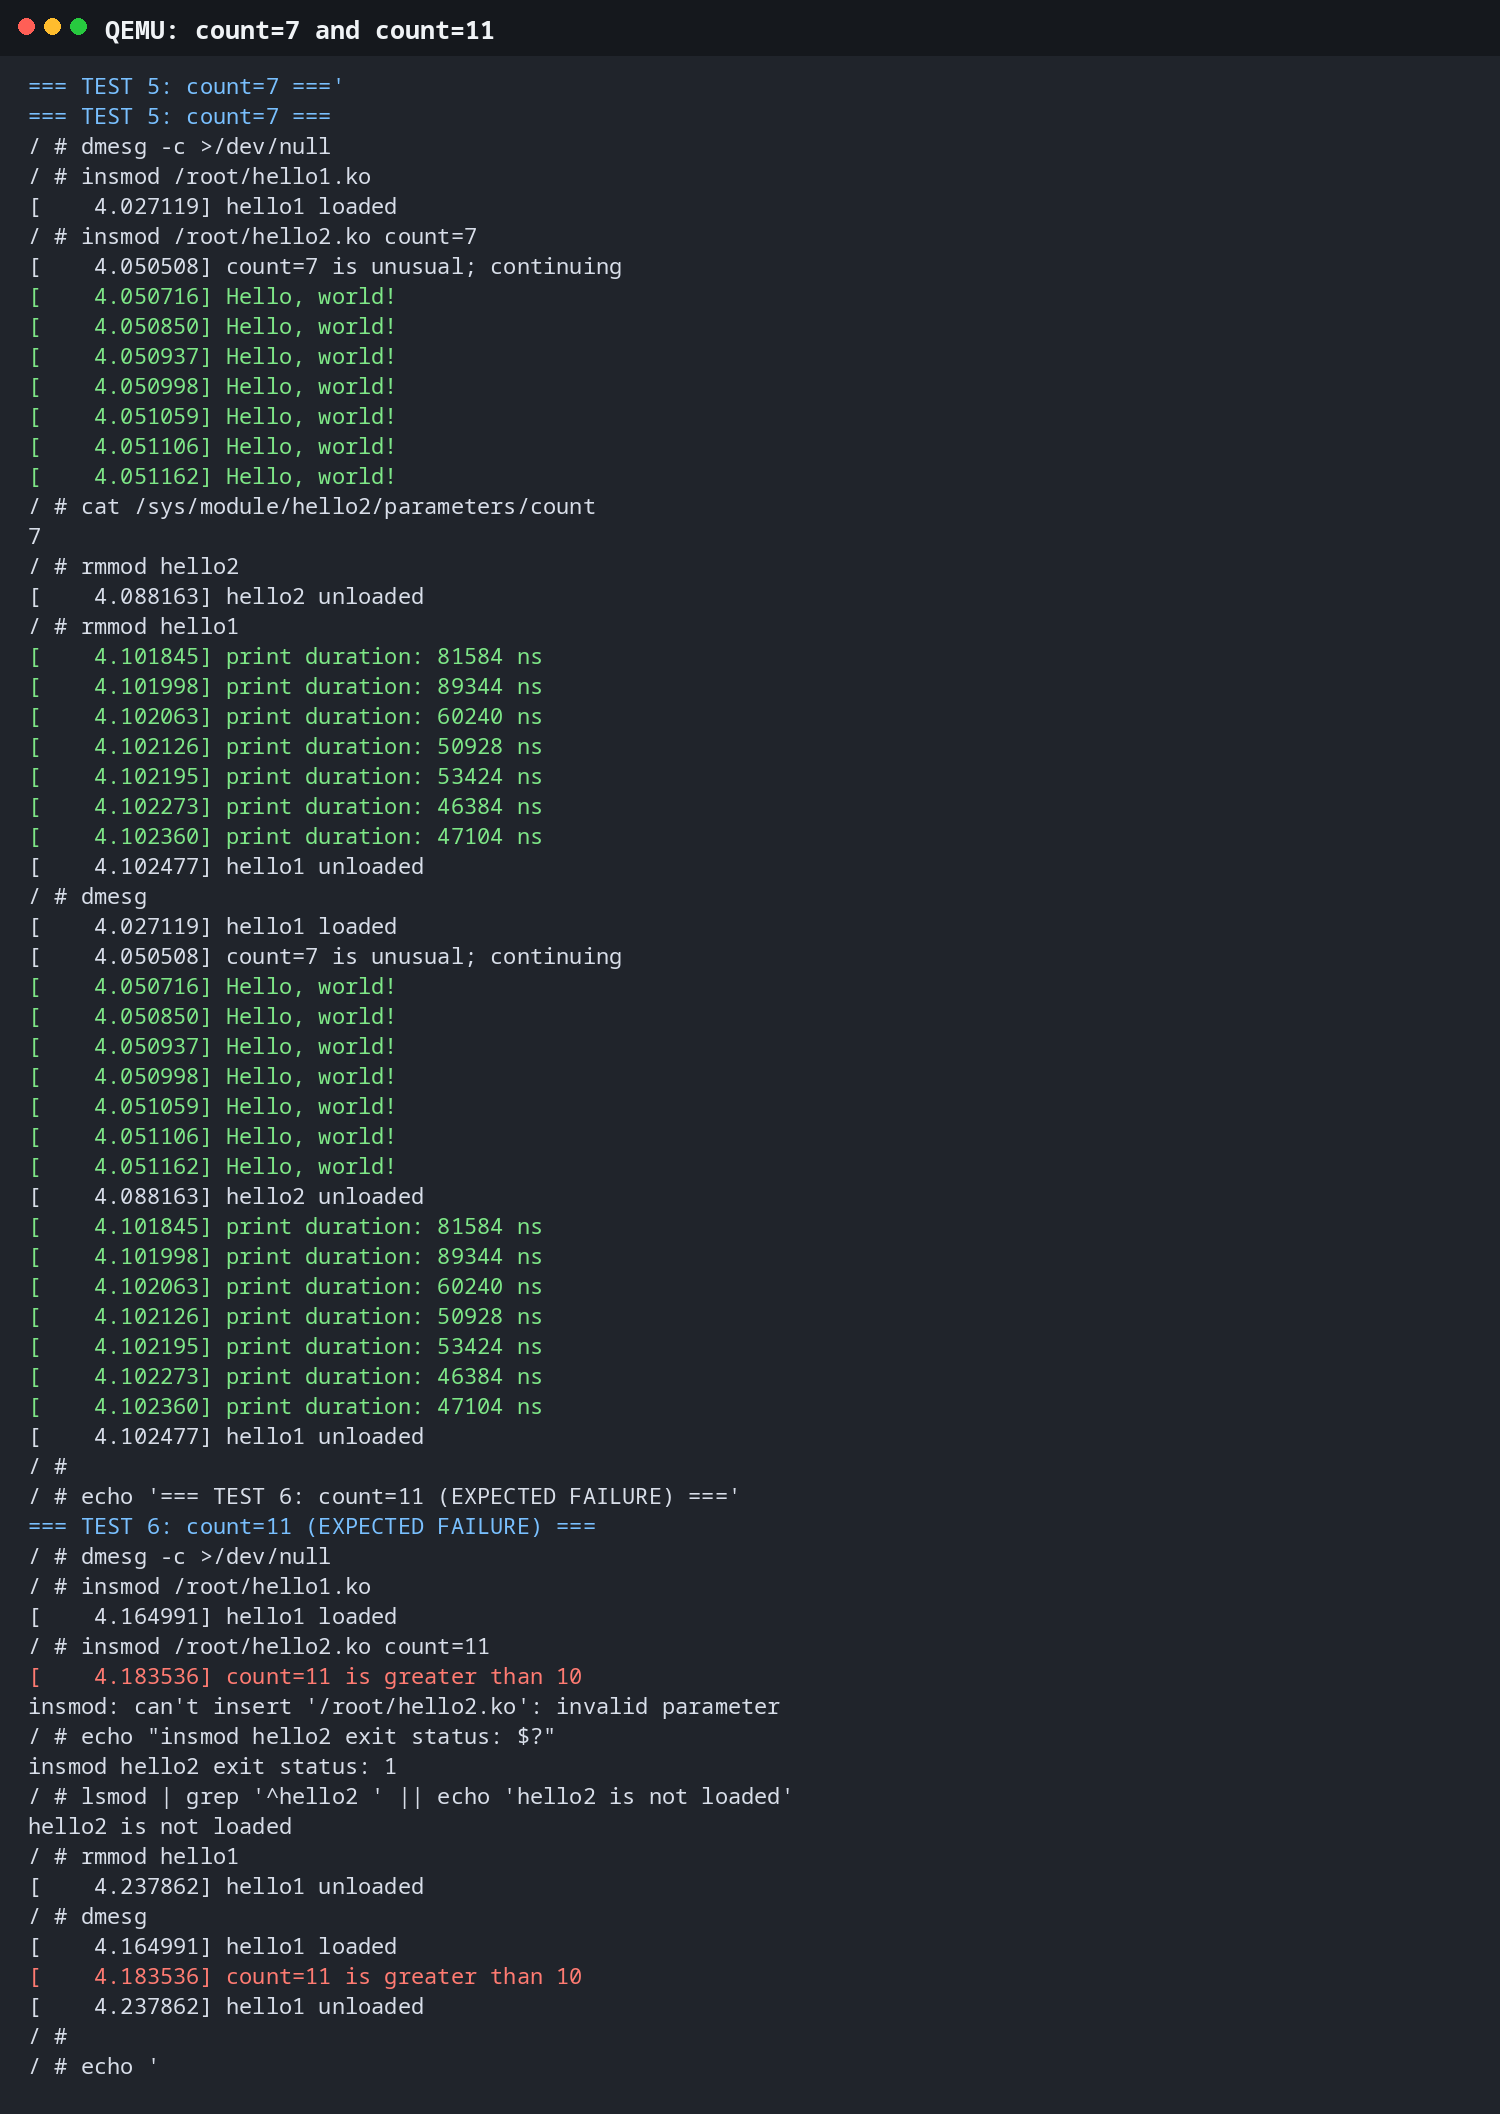
\includegraphics[width=0.64\textwidth]{media/parameters-7-11.png}
  \caption{Попередження для count=7 та відмова для count=11}
\end{figure}

Під час \texttt{rmmod hello1} кількість рядків
\texttt{print duration: ... ns} збігалася з кількістю викликів
\texttt{print\_hello()}. Це підтверджує правильну роботу списку, обох
часових міток і звільнення елементів. Повний вивід збережено у форматах
TXT і HTML у каталозі \texttt{evidence}.

\section{Висновки}

У роботі реалізацію з ЛР №4 розділено на два зовнішні модулі ядра.
\texttt{hello1} експортує сервіс друку, зберігає події у двозв'язному
списку та вимірює тривалість кожного виклику. \texttt{hello2} залежить від
першого модуля, приймає параметр \texttt{count} і викликає експортовану
функцію.

Модулі пройшли \texttt{checkpatch.pl} без помилок і попереджень, були
зібрані для ARMv7 та перевірені у QEMU. Практично підтверджено поле
\texttt{depends: hello1}, помилку невизначеного символу при неправильному
порядку завантаження, роботу параметра через sysfs і всі рівні повідомлень
\texttt{pr\_info}, \texttt{pr\_warn}, \texttt{pr\_err}.

\section*{Використані матеріали}

\begin{enumerate}[leftmargin=*]
  \item Методичні вказівки до лабораторної роботи №5.
  \item Вихідний код Linux 4.19.325: \path{include/linux/printk.h}.
  \item Документація Kbuild: \path{Documentation/kbuild/modules.txt}.
  \item Результати збирання ядра та initramfs із лабораторної роботи №3.
\end{enumerate}

\newpage
\section*{Додаток А. Вихідний код hello1.c}
\addcontentsline{toc}{section}{Додаток А. Вихідний код hello1.c}

\VerbatimInput[fontsize=\tiny,breaklines=true,breakanywhere=true,frame=single,framesep=2mm]{../src/hello1.c}

\newpage
\section*{Додаток Б. Вихідний код hello2.c}
\addcontentsline{toc}{section}{Додаток Б. Вихідний код hello2.c}

\VerbatimInput[fontsize=\tiny,breaklines=true,breakanywhere=true,frame=single,framesep=2mm]{../src/hello2.c}

\section*{Додаток В. Заголовок і Kbuild}
\addcontentsline{toc}{section}{Додаток В. Заголовок і Kbuild}

\VerbatimInput[fontsize=\small,frame=single,framesep=2mm]{../src/inc/hello1.h}
\VerbatimInput[fontsize=\small,frame=single,framesep=2mm]{../src/Kbuild}

\end{document}
